\chapter{Evaluation}
\label{ch:evaluation}

This chapter discusses three different experiments that are conducted to check for effectiveness and efficiency of RDF-Doctor.
First experiment checks the effectiveness of RDF-Doctor against set of test cases provided in~\cite{TurtleTests:Online}.
In the second experiment, a random number of errors is generated using a Poisson Distribution for a period of eight instances of time while a Uniform Distribution randomly selects types of errors for each instance of time, respectively.
%number generators for a period of time of 8 time instances to simulate a couple of syntax errors, produced by an ontology user, 
Finally, the efficiency of RDF-Doctor is measured when both, the number of errors and the size of ontologies are changed. 

In the following sections, three experiments designed to evaluate RDF-Doctor are presented. 
Each section describes a particular experiment by giving its objective, presenting the followed procedure, and discussing the achieved results.

\section{Experiment Configuration}

All experiments are run on a Linux Ubuntu 18.04 machine with a 4th Gen Intel Core i5-4300U CPU, 3MB Cache, 2.90GHz with 8GB RAM 1333MHz DDR3. 
RDF-Doctor is implemented using Java version 9. 
ANTLR framework version 4.7.1 is used to build the internal parser in RDF-Doctor.%, as well, as an imported library for compiling and running of it.  

\section{Experiment I} 
In this experiment, RDF-Doctor was validated against RDF Suite Test, specifically Turtle serialization. 
%Next text discusses the objective, shows the procedure, and finally, presents and discusses the result.  

\subsection{Objective}

There exists a number of Test Suites for each RDF serializations which are recommended by W3 Consortium (W3C) in ~\cite{TurtleTests:Online}.
%The evaluation phase starts with where a Test Suite defined in the Turtle serialization. 
These Test Suites can be used to check for the proficiency of a parser with respect to a certain serialization.% can be validated with these files found in a corresponding Test Suite. 
Therefore, the target of this experiment is to measure the proficiency of RDF-Doctor while testing with the W3C Turtle Test Suite.

\subsection{Procedure}

\begin{table}[]
\centering
\begin{tabular}{|l|l|l|l|}
\hline
\begin{tabular}[c]{@{}l@{}}File Content \end{tabular} & Detected  & Not detected & Total \\ \hline
 Correct Syntax              &      185    &      25  & 210 \\ \hline
 Incorrect/Bad Syntax              &      53    &    12  & 65 \\ \hline
 Total            &      238   &       37 & 275  \\ \hline
\end{tabular}
\caption{\textbf{Evaluation summary of RDF-Doctor for both correct and incorrect syntactic forms.} "Detected" for Correct Syntax means that RDF-Doctor is able to recognize them as correct syntactic forms, whereas, for those which are not correctly recognized classified under "Not detected", similarly, "Detected" in Incorrect/Bad Syntax referred to recognized syntactic forms  as incorrect forms with releasing corresponding error messages, but "Not detected" specifies  incorrect syntactic forms  which are not recognized and might generate false positives.}
\label{tab:TurtleSuit}
\end{table}

%Files at \cite{TurtleTests:Online} were prompted to validate a parser that parses a Turtle serialization, hence, it was used to test RDF-Doctor. 
The total number of files of the W3C Test Suite is 275, which we divided in two parts: 1) files that are syntactically correct; and 2) files that are syntactically incorrect.
The first subset contains 210 correct files, whereas the second one contains 65 files, as represented in Table \ref{tab:TurtleSuit}.
We computed the Precision and Recall, donated by equations \ref{eq:1} and \ref{eq:1}, to calculate the percentage of errors which are correctly flagged as syntax errors, and calculate the percentage of actual syntax errors which are correctly recognized, respectively. 

%For evaluation, the precision and recall are computed using the equations \ref{eq:1} and \ref{eq:2} respectively.  
\begin{align} 
   Precision=  \frac{t_p}{t_p+f_p}\,;\qquad
\qquad\parbox{4.0cm}{\footnotesize$\begin{aligned} t_p &= \text{ number of true positives}\\[-1.0ex] f_p &= \text{ number of false positives}\end{aligned}$}
   \label{eq:1}
\end{align}
\begin{align}
   Recall =  \frac{t_p}{t_p+f_n} \,;\qquad
\qquad\parbox{4.0cm}{\footnotesize$\begin{aligned} t_p &= \text{ number of true positives}\\[-1.0ex] f_n &= \text{ number of true negatives}\end{aligned}$}
   \label{eq:2}
\end{align}

 
\begin{table}[]
\centering
\begin{tabular}{|l|l|l|l|}
\hline
\begin{tabular}[c]{@{}l@{}}Classification of Error Types\end{tabular} & Detected & \begin{tabular}[c]{@{}l@{}}Not detected\end{tabular} & Total \\ \hline
 Escape Characters              &      0    &    4 &   4  \\ \hline
 Bad Keywords             &      5   &    0 &   5  \\ \hline
 Bad Literals with langTag             &      2   &    0 &   2  \\ \hline
 Bad Local Name-space in IRI             &      2   &    3  &   5  \\ \hline
 Bad Namespace in IRI             &      2   &    0 &   2  \\ \hline
 N3 Extra             &      11   &    1 &   12  \\ \hline
 Bad Namespace in Directives             &      2   &    0 &   2  \\ \hline
 Bad Number as a Literal             &      5   &    0 &   5  \\ \hline
 Bad Directives             &      4   &    0 &   4  \\ \hline
 Bad Strings             &      6   &    1 &   7  \\ \hline
 Bad Structures            &      12   &    0 &   12  \\ \hline
 Bad IRI            &      2   &    3 &   5  \\ \hline
 Total            &      53   &    12 &   65  \\ \hline
\end{tabular}
\caption{\textbf{Evaluation of RDF-Doctor against detection of incorrect syntactic forms in Turtle Test Suite \cite{TurtleTests:Online}.} The test focuses on the files, including  an incorrect Turtle syntax,  ”Detected” in pointed to recognized syntactic forms as incorrect forms with releasing corresponding error messages, but ”Not detected” specifies incorrect syntactic forms which are not recognized and might generate false positives.}
\label{tab:detection}
\end{table}

\subsection{Result and Discussion}

%The test drives the result when dealing with either correct or incorrect Turtle syntax. 
%While trying correct syntaxes should be recognized as correct, similarly in case of incorrect syntaxes plus exception errors should be fired.  
As we can observe from results given in Table \ref{tab:TurtleSuit}, the majority of syntactically correct files, i.e. 88\%, are categorized correctly, i.e., as free of errors, while the remaining 12\% are considered as syntactically incorrect.
%mostly of correct syntaxes with 88\%, while the remaining 12\% RDF-Doctor are not recognized and it consider them as errors. 
On the other hand, when dealing with incorrect syntaxes, results show that 81,5\% of files which include incorrect syntaxes are detected and the appropriate error message is given, whereas the rest 17,5\%, are not recognized as errors, thus no error message is given\todo{where are precesion and recall calculated, please add them}.
\floatstyle{plain}
\restylefloat{figure}
\begin{figure}
\begin{center}
		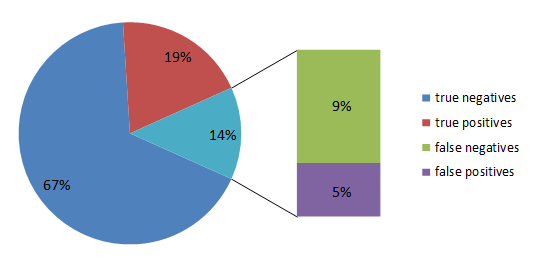
\includegraphics[scale=0.6,angle=0,trim=4 4 4 4,clip]{images/Experiment01.png}
		\caption{\textbf{RDF-Doctor evaluation with Turtle Test Suite \cite{TurtleTests:Online}.} Each file in \cite{TurtleTests:Online} was classified of having a syntax error or not and then the final result was grouped into 4 categories: true positives (files with syntax errors are correctly identified); false positives (files without syntax errors are incorrectly identified); false negatives (files with syntax errors are incorrectly rejected); true negatives (files without syntax errors are correctly rejected).}
		\label{Fig:Experiment01}
\end{center}
\end{figure}


\section{Experiment II}

In the following, we provide details about second experiment where RDF-Doctor is validated through a synthetic experiment. 

\subsection{Objective}
With the objective of simulating a real world scenario where an ontology engineer develop an ontology for a particular domain using a plain text editor.
During a working which commonly has eight hours, the engineer may perform several changes to the ontology, while saving it for each hour.
While doing that, the engineer may introduce a number of syntactic errors, which he has to identify and correct them, before being able to share his contribution with other team members.
%To get rid of the generated bias, this experiment uses both Poisson distribution and uniform random number generation methods. It also assumes a naive user editing an RDF input data, found in an environment similar to the one in Figure \ref{Fig:Motivation} and he is mistakenly generating some  syntax errors. Then, the inserted syntax errors evaluate the quality of RDF-doctor.


\subsection{Procedure}

In this experiment, we assume that, while the ontology engineer contributing to the DBpedia ontology, he performs several modifications, e.g. insert, edit or delete during a period of eight instances of time, i.e., each hour. 
The Poisson and Uniform Distribution are used to simulate the number and the type of errors occurred in each instance of time, respectively.
The average number of syntax errors per instance of time is represented by $\lambda$ parameter. 
For example, $\lambda$ = 5, means that five syntax errors are occurred per hour in average.  
%As an input for a Poisson distribution, 10 syntax errors per instance of time was supplied. 
The Uniform Distribution is used to randomly select the error types from a comprehensive list of errors as given in Appendix~\ref{tab:syntaxErrorCate}.
%Hence, for each instance of time we calculate value of $\lambda$, then the output value drives how many number of syntax errors are entitled for that instance of time.
%Next, Those syntax errors are arbitrarily selected from the type of errors range [1-61], drawn by rows of Table . 
Moreover, the exact location for injecting syntax errors within the RDF file is realized using the Uniform Distribution where a random line number is generated.
The error is successfully applied, if the randomly selected location is appropriate for the error type, otherwise, one of the lines for its neighborhood is selected. 
In case the error is related to the header, then the injection is applied into Prefix and Base directives.  

\begin{figure}[ht]
	\begin{center}
		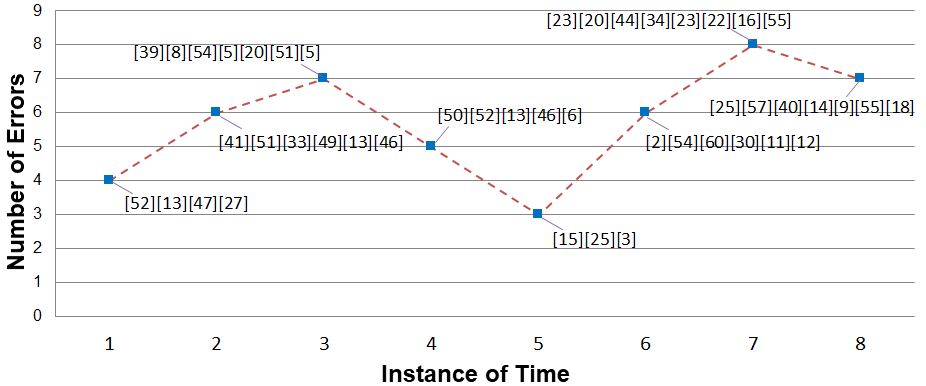
\includegraphics[scale=0.45,angle=0]{images/Experiment02-01.png}
		\setlength\belowcaptionskip{-5mm}
		\caption{\textbf{The distribution of syntax errors.} Number and types of syntax errors between brackets for an interval of eight instances of time. 
		A Poisson Distribution with the parameter $\lambda$ = 5 models an average of five syntax errors per instance of time. 
		Each instance of time shows value of $\lambda$, assuming the ontology engineer can generate between 1 to 10 syntax errors per instance of time. 
		Also, a Uniform Distribution generates random numbers in the interval between 1 and 61, to select the error type as listed Appendix~\ref{ch:synErrCategories}. 
		For example, at the 5\textsuperscript{th} instance of time, three error types are introduced, i.e., [3,15,25].} 
		\label{Fig:experiment2}
	\end{center}
\end{figure}


	\begin{figure}[ht]
	\begin{center}
		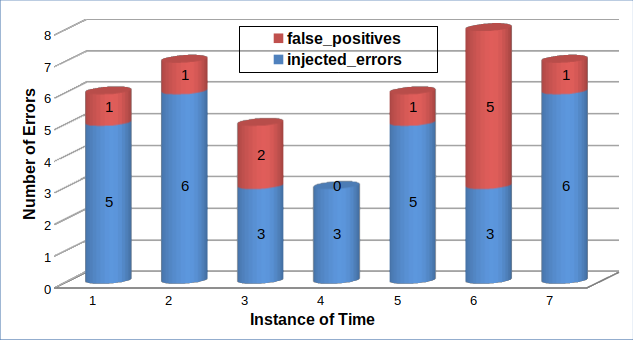
\includegraphics[scale=0.3,angle=0]{images/Experiment02-02.png}
		\setlength\belowcaptionskip{-5mm}
		\caption{\textbf{Error detection when syntax errors are randomly distributed.} 
		For each instance of time, a number of errors which are detected or not detected by RDF-Doctor are shown.
		%"detected", and those one which were undetected and unrecognized by RDF-Doctor, referred as "undetected".
		} 
		\label{Fig:Experiment02-02}
	\end{center}
\end{figure}

\subsection{Result and Discussion}

Experimental results illustrated in Figure \ref{Fig:Experiment02-02} shows that RDF-Doctor in majority of the cases is able to correctly recognize syntax errors. 
More specifically, in half of the instances time, appart from one syntax error not recognized, all of them are identified.
In time instance five, all errors are detected.
However, there are some instances of time where more than one error is not recognized, such as time instance number 6\textsuperscript{th} with five undetected syntax errors.
This can be due to fall most of the unrecognized syntax errors in this time instance since the insertion of the syntax errors was done randomly{this sentence is not clear, and you have to give a better reason, not only saying that they are generated randomly, bcz this applies for all}.

Figure \ref{Fig:Experiment02-03} illustrates a comparison of the number of the injected errors versus the number of false positives of this experiment. 
As we can observe, the number of false positive is higher than actual errors which may result due the probability of existing one or more unrecognized syntax errors which are coming from the libraries of the ANTLR framework. 
One possible solution for this is by optimizing RDF-Doctor with developing an additional layer to internally handle these type of errors, besides the error specification in production rules for a particular grammar.

%rest of the times instances show zero or few errors, except the time instance number 6\textsuperscript{th}, , this can be due to fall most of the unrecognized syntax errors in this time instance since the insertion of the syntax errors was done randomly.  

\begin{figure}[ht]
	\begin{center}
		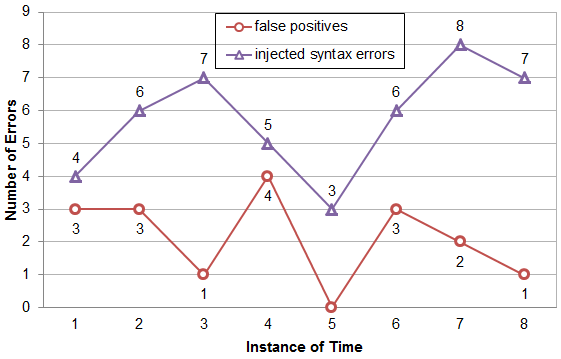
\includegraphics[scale=0.7,angle=0]{images/Experiment02-03.png}
				\setlength\belowcaptionskip{-5mm}
		\caption{\textbf{Result of false positives during RDF-Doctor validating with randomly distributed syntax errors.} 
		For each time instance, when number of syntax errors are randomly inserted, that may result in false positives since one of the unrecognized syntax errors can be in-between those inserted ones.} 
		\label{Fig:Experiment02-03}
				\setlength\belowcaptionskip{-5mm}
		\setlength\abovecaptionskip{0mm}
	\end{center}
\end{figure}
 


\section{Experiment III}

This experiment evaluates the behaviour and the performance RDF-Doctor by changing the number of syntax errors and the size of ontologies. 

\subsection{Objective}
With the objective of checking the effect on the behaviour and the performance of our approach whenever the number of errors increases.
Furthermore, we evaluate the performance of RDF-Doctor when the size of the ontologies is changed, to simulate real world scenarios where ontologies continue growing over the time.

%We are studying the effect of growing of number of syntax errors, as well as, the size of ontologies when it is changed. 


\subsection{Procedure}

We used two types of ontologies: small; and medium sized. 
The Friend of a Friend Vocabulary (FOAF)\footnote{\url{http://www.foaf-project.org/}} is used as a small ontology with total number of 631 triples. 
As a medium sized ontology, we used DBpedia\footnote{\url{https://wiki.dbpedia.org/develop/datasets/dbpedia-version-2016-10}}, version 2016-10, with a total number of 30,790 triples. 
In both ontologies were three different numbers of syntax errors are introduces, i.e., 10, 30, 61 syntax errors are randomly injected using the same procedure where the Uniform Distribution is utilized.
Additionally, to avoid any impact on the current overload of the processor during the execution time, we run our experiment five times for each case, and calculate the average processing time.

 
\subsection{Result and Discussion}

Figure \ref{Fig:Experiment03-01} illustrates the performance of the number of errors and the ontology size. 
When introducing 10 syntax errors, 9 out of 10 are detected and one is not detected for both, FOAF and DBpedia ontologies, respectively. 
In the second case, 25 out of 30 injected errors are detected in FOAF and 26 out of 30 from injected errors in DBpedia are detected. 
Finally, from 61 injected errors, 6 in FOAF and 11 DBpedia, are not detected.
In all cases, for each error that is detected an expressive message is given to help users to resolve them. 

\begin{figure}[ht]
\begin{center}
		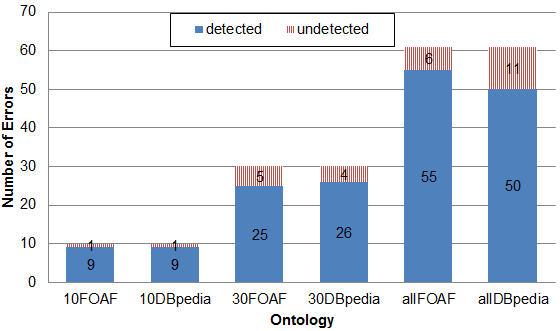
\includegraphics[scale=0.3,angle=0]{images/Experiment03-01.png}
				\setlength\belowcaptionskip{-5mm}
		\caption{\textbf{Impact of number of errors and the size on error detection.} 
		FOAF and DBpedia ontologies are used to evaluate RDF-Doctor, 10foaf, 30foaf, allfoaf are datasets of FOAF ontology, including with 10, 30, 61 random syntax errors, respectively, same is applicable for DBpedia. Detected errors are the errors which were properly identified by RDF-Doctor and the matched error messages were released, while undetected errors are those which not correctly recognized.}
		\label{Fig:Experiment03-01}

\end{center}
\end{figure}


Another essential point is number of false positives as shown in Figure \ref{Fig:Experiment03-02}. 
It can be seen that the false positives are incremented while raising of the number of syntax errors.
This comes as consequence of increasing number of unrecognized syntax errors, forcing the parser to try to recover from such errors by adding or removing some tokens, which in turn produces an increased number false positive errors.   

\begin{figure}[ht]
\begin{center}
		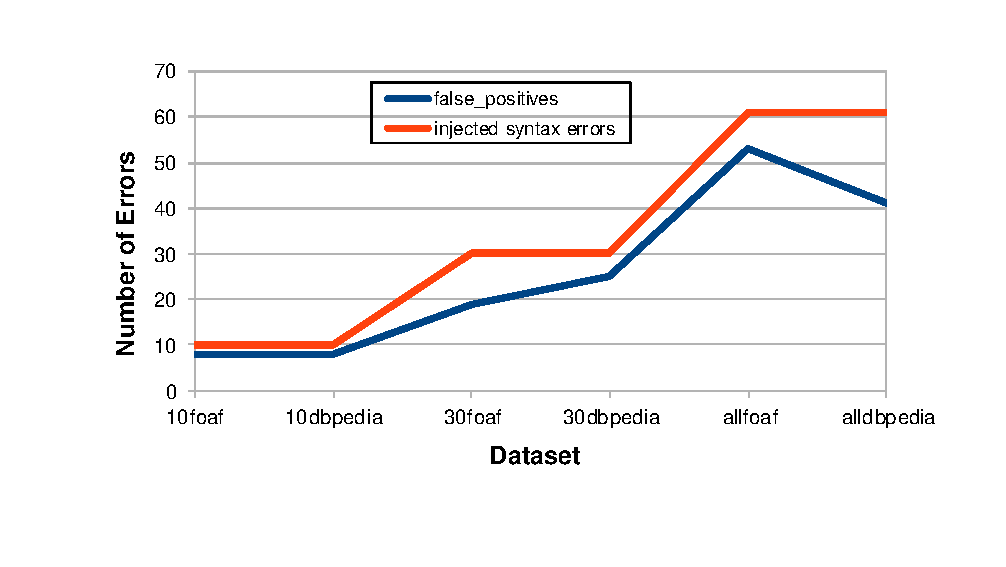
\includegraphics[scale=0.8,angle=0]{images/Experiment03-02.pdf}
		\setlength\belowcaptionskip{-5mm}
		\setlength\abovecaptionskip{-10mm}
		\caption{\textbf{Result of false positives when number of errors and ontology size are increased.} Unrecognized errors may generate more false positive errors than actual errors. 
		%and when the number of errors increase, the false positives are comparably increased.
		}
   \label{Fig:Experiment03-02}
\end{center}
\end{figure}

The performance of RDF-Doctor is presented in Figure \ref{Fig:Experiment03-03}. 
It summarizes the impact of both, the number of errors and the ontology size on the RDF-Doctor performance.
As we can observe, the numbers of errors has no influence on the performance, i.e., the processing time is similar in either FOAF or DBpedia while changing number of errors. 
On the other hand, the size of ontologies has a high impact on the overall performance, i.e, processing DBpedia consumes about 29000ms in average, whereas, FOAF is parsed in about 2000ms.   
As a conclusion to this experiment, approximately more than 90\% of injected syntax errors are detected, as shown in Figure~\ref{Fig:Experiment03-01}. 
%Also, number of false positives can be improved if RDF-Doctor recognized those undetected errors by either do more laboratory works to match those patterns or may with the new versions of ANTLR library.  
%talk about the correction of errors #numbers 

\begin{figure}[ht]
\begin{center}
		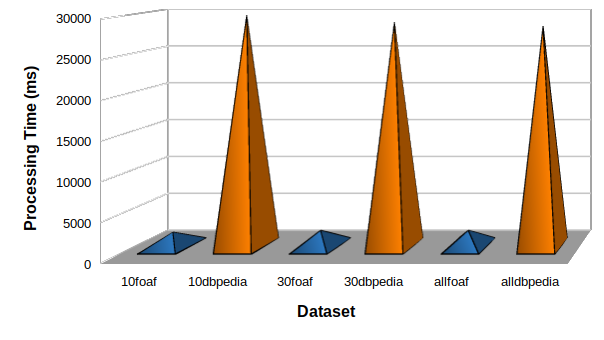
\includegraphics[scale=0.7,angle=0]{images/Experiment03-03.png}
		\setlength\belowcaptionskip{-5mm}
		\setlength\abovecaptionskip{0mm}
		\caption{\textbf{Performance evaluation when number of errors and ontology size is changes, respectively.} 
		Performance is calculated with required processing time, i.e., in miliseconds (ms) in both cases: 1) 10, 30, and 61 injected syntax errors; 2) FOAF ontology with 631 triples and DBpedia ontology, with 30,790 triples.}
\label{Fig:Experiment03-03}

\end{center}
\end{figure}
